\chapter{Plan of Work}

\section{Development and Report Milestones}

Illustrated on the next page is a gantt chart reflecting our goals relative
to the project deadlines. It incorporates both core development and report items.
For our initial stages we focus on environment and platform set-up (i.e.
deploying a development webserver) and the initial, core code implementation. At
the same time we will finalize the details of our final product via the report
milestones. \\ 

{\bfseries Development milestones} have been spread out following the completion 
of the first report on 22 February 2013, beginning with deploying our development
 environment and server through Heroku from which we continue to our next 
 milestone of deploying Ruby on Rails as well as all the Gems and API packages we are incorporating into our project, most notably Yahoo! Finance. \\

{\bfseries Report milestones} are also set concurrently. As we begin to initialize
our development environment, we will also build on top of and expand on previous
reports to expand upon and fully realize the details of {\textit Capital Games}.

%{\bfseries Core goals leading up to Demo 1} include establishing all core 
%functionality for {\textit Capital Games}. This includes the following:
%\begin{itemize}
%\item {\bfseries Rails framework-deployed core functionality :} This
%includes a working system for navigating the website, registering a new
%user account, logging in, and creating as well as participating in leagues.
%\item {\bfseries Setting a foundation for the database: } On top of having 
%the aforementioned core functionalities, they also must be able to pass
%data through a routed database.  
%\item {\bfseries Implementing the Yahoo! Finance API: }
%\item {\bfseries A functional user interface:} Our website should be useable, 
%and having a functional user interface from the start will give us a lot of
%room to expand and optimize the UI. \\
%\end{itemize}


\section{Breakdown of Responsibilities}

Contributions leading up to the completion of this report are covered in the 
"Contributions" table on the page following the gantt chart. For the future
division of labor, we all plan on subdividing aspects of both the next reports 
as well as the development of the {\textit Capital Games} Alpha. 

Responsibilities for server/development environment deployment and set-up will be shared between Val and both Jeffs, as all three equally have great experience in the subject. Meanwhile Nick, and Eric will work of sequence diagrams.

While all other diagrams on the report will be covered by both Jeffs, the User Interface Design and Implementation will be worked on by Val, Dario, and Eric. Nick and Dario will work on both data types and operations while Val and Eric also
 work on the traceability matrix. 

System architecture and design will be covered by Nick and Val. Jeff R. and Dario will begin on the database structure and site routing via the Rails framework. Nick and Jeff A. will work on the implementation of users in the meantime.

From there we will further subdivide work on the final aspects of the website, likely sticking with our initial idea of splitting predominant responsibilities between model, view, and controller aspects (MVC). Jeff R. and Jeff A. will work on the Model aspect, Dario and Eric will work on the views aspect, and Nick and Val will focus on the controller aspect.

\hfil\eject \pdfpagewidth=8.5in \pdfpageheight=16in
\begin{figure}
\centering
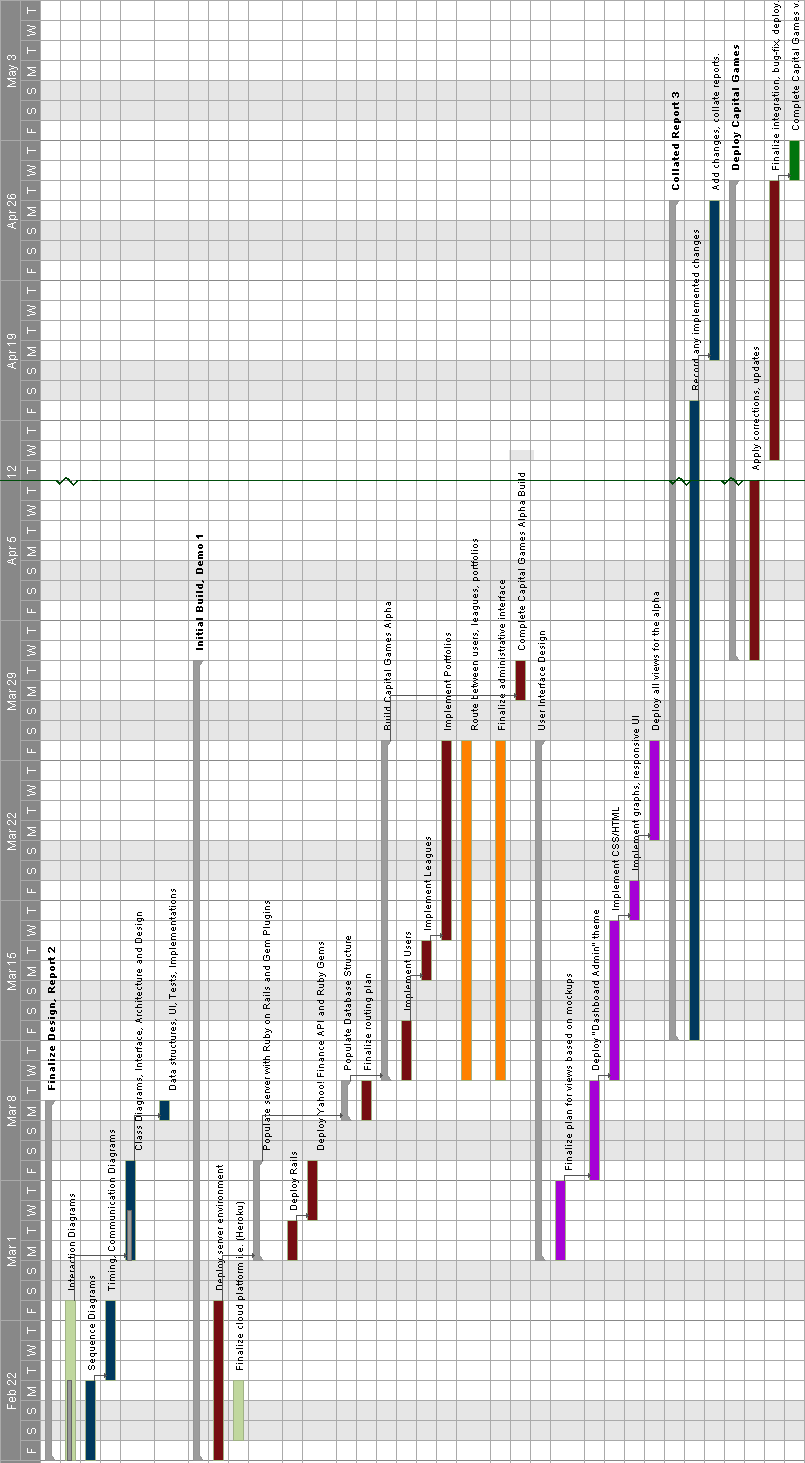
\includegraphics[width=7in]{./img/gantt.png}
\caption{(Note: Best viewed at 100\%) This gantt chart projects how we will concurrently work on
the project. All blue items are report-related, red and orange relate
to the core project development and purple illustrates UI milestones.}
\end{figure}
% This chapter should include a Gantt chart for each our
% coding timelines for the first and second report and
% maybe even a second Gantt chart for our report deadlines
% from this report through May.
%
% Remember that we're trying to roll out core functionality 
% in time for the first demo, so try to include as much as 
% possible about creating users, leagues, basic settings (only),
% most trade and search things on the part for the first report,
% and the comments, reporting, adjusting settings, begin/end dates,
% privacy, mailing, whatever for the second. See our proposal for 
% the laundry list of features we actually said we'd be delivering.
%
% Also maybe talk about "Project Ownership", since he's big 
% on that. 
